

%Results should be clearly displayed and should provide a suitable representation of your results for the points you wish to make. Graphs should be labeled in a legible font and if more than one result is displayed on the same graph then these should be clearly marked.   Please choose carefully rather than presenting every results. Too much information is hard to read and often hides the key information you wish to present. Make use of statistical methods when presenting results, where possible to strengthen the results.  Further, the format of the presentation of results should be chosen based on what issues in the results you wish to highlight. You may wish to present a subset in the experimental section and provide additional results in the appendix.

\subsection{Experimental Results}
\label{subsec:parameterSettings_results}

Table \vref{table:parameterSettings2} presents the parameters and candidate values tested, in addition the selected value for each parameter. The complete experimental steps with the corresponding results can be found in, Appendix \ref{appendixC}, Table \vref{table:pm1} and Table \vref{table:pm2}. 

    \begin{table}[H]
    \centering
    \begin{tabular}{|l|l||l|}
    \hline
    \textbf{Parameter} & \textbf{Candidate values} & \textbf{Selected value}\\
    \hline
    $s$ & 10, 50, 100, 125 & 50 \\
    $i$ & 10, 50 , 100, 125 & 125\\
    $E$ & 10\%, 25\% 50\%, 90\% & 25\% \\
    $CA$ & 0\%, 5\%, 10\%, 25\%, 50\%, 100\% & 25\% \\
    $AF$ & 0\%, 5\%, 10\%, 25\%, 50\%, 100\% & 5\% \\
    $p_{b}$ & 0.0, 0.1, 0.5, 0.9, 1.3 & 1.3 \\
    \hline
    \end{tabular}
    \caption {Results from the parameter settings experiment}
    \label{table:parameterSettings2}
    \end{table}
    
\subsubsection*{Selecting final parameters}

The computed Confidence Interval does not become remarkably better after running the proposed system 50 times, compared to 30 times. Produced results regarding parameters run 30 times can therefore be considered valid.
\newline
%Because our confidence coefficient is sat to correspond to 95\%, we are able to say that we are 95\% confident that the true population parameter is between the lower and upper calculated values.

As one can observe in Table \vref{table:pm1}, increasing parameters $s$ and $i$ both decrease the $TOTFIT$ value. One aspect not considered in the initial parameter setting experiment is that the size of $s$ and $i$ affects each other. A colony of 50 ants with 125 iterations produce close to similar results to 125 ants with 50 iterations, due to the fact that the total number of ants traversing the network will be approximately the same. The most optimal would therefore be to observe the results when increasing the value of these parameters together. However, an increase in the swarm size or number of iterations both clearly affect the computational cost of the proposed system. The average runtime of each run, with candidate values of 50 and 125, is presented in Table \vref{table:svsiruntime}. As one can see, there is a difference in the running time with a colony size of 125 versus 125 iterations. Because the proposed system is going to be run an excessive amount of times when testing performance, increasing both of these parameter values will result in an enlarged runtime. As seen in Table \ref{table:pm1}, the value of 125 iterations produce better results than a colony size of 125. Due to the runtime difference and the produced results, the selected value of parameter $s$ is sat to \textit{50} and $i$ is sat to \textit{125}.

\begin{table}[H]
    \centering
    \begin{tabular}{|l|l|l|}
    \hline
    \textbf{Candidate value} & \textbf{$s$} & \textbf{$i$}\\
    \hline
    50 & 181.9 & 187.7 \\
    100 & 883 & 756\\
    \hline
    \end{tabular}
    \caption {Running time in seconds for different candidate values of parameters $s$ and $i$}
    \label{table:svsiruntime}
    \end{table}

%It is worth mentioning that values below 50 of parameter $s$, sometimes produce ant colonies were no ants satisfies the initial Constraint \ref{itm:criteriaConnectedGraph} described in Section \ref{sec:algoConstraints}. When $s$ is 10, this occurs on average 14.5\% of the iterations. If no ant satisfy the initial constraint, no ant is either evaluated, and their results will be invalid. 

%\citet{poorzahedy11} reports that ``In more than 80\% of the time, the best found solution of the problem has been found in less than 65 iterations'' --> Settes i sammenheng med $i$.

%\begin{figure}[H]
%\begin{center}
 % 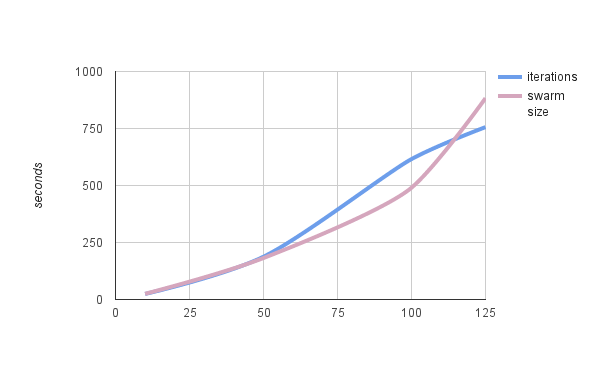
\includegraphics[width=5in]{assets/iterations_swarmsize_runtime.png}
  %\end{center}
  %\caption{Comparing Runtime when increasing the Swarm Size and the Number of Iterations}
  %\label{fig:svsiruntime} 
%\end{figure}

Observing the produced results of parameter $E$ in Table \vref{table:pm1}, evaporating 25\% of the pheromone each iteration gave the best average total fitness, closely followed by 50\%. The fact that a noticeable amount of pheromone evaporates each iteration is beneficial. However, removing over 90\% at each iteration is an excessive amount. The worst results were achieved when $E$ is 10\%. Evaporating only a small percentage of the pheromone may result in ants getting stuck at local optima, due to the fact that routes found in the early iterations will contain significantly more pheromone than newly discovered routes. Evaporation is important when it ensures that the pheromone level on routes explored in early iterations, but later discarded in favor of others, decreases. By stating $E$ as a percentage an equivalent amount of pheromone is removed from each edge, independent of whether the pheromone level is big or small. 
\newline

Parameter $CA$ produced best results with a value of 25\%, meaning there is a 25\% probability in that an ant is declared ``crazy'' in the beginning of each iteration. As mentioned, a ``crazy ant'' makes completely random decisions and select edges regardless of the pheromone value. $CA$ will decrease at each iteration based on the Inertia Weight, as described in Section \vref{sec:algoGeneratingSuperSwarm}. The results in Table \vref{table:pm2} shows that the algorithm benefits from the fact that some ants are declared crazy. As stated in Section \vref{section:methodDescription}, if some ants are declared crazy, the probability of getting stuck at a local optima may decrease. However, if the value is greater than 25\%, the average $TOTFIT$ results worsen. Not surprisingly, is this because half or more of the colony acts completely random, and the algorithm looses some of the performing boosting features from ACO, such as favoring edges frequently walked by other ants. 
\newline

The amount of $AF$ determines the amount of Following Ants ($FA$) in the next iteration, and the $FA$ follow the same path as the best ants' paths unconditionally. Observing the results obtained in Table \vref{table:pm2}, the $TOTFIT$ value deteriorates when the amount of $AF$ becomes greater than 25\%. When the amount of $FA$ becomes too great, a relatively large number of normal ants will not be able to explore new (possibly better) routes in the next iterations, and the algorithm may not be able to escape from a local optima. But as one also can see, increasing the value computes better results than 0\%. Rewarding some good route sets seems to boost the algorithms performance, and 5\% is selected as the final parameter for $AF$. 

The value of $p_b$ is as mentioned strongly dependent on the value of $AF$. This is due to the fact that the more following ants, the more pheromone added to each edge in the best route sets. The values of $p_b$ are therefore tested with the selected value of $AF$. As one can observe in Table \vref{table:pm2}, the proposed system's performance increase in line with the value of $p_b$. The relatively small amount of edges selected by $AF$ benefit from granting these edges in the best routes with extra pheromone. %However it seems that when $p_b$ becomes greater than 0.9, the $TOTFIT$ value worsen. This may be because the amount of pheromone wil

